\chapter{FROM OVERLAYS TO SECURE VIRTUAL PRIVATE NETWORKS}
\label{chap:security}

In this chapter, I take the results from Chapter~\ref{chap:bootstrapping} and
apply them to IPOP~\cite{ipop} in order to construct a fully decentralized P2P
VPN (peer-to-peer virtual private network).  While sharing overlays in IPOP
makes for simplified use of the system, in reality, it introduces significant
security challenges.  For example, a misconfigured or malicious peer could
potentially disable the entire overlay, rendering all VNs (virtual networks)
useless.  If security and hence isolation is important, prior to VN deployment,
a user would need to deploy a secure overlay and configure their VPN to
bootstrap from it, given the complexity many users may reconsider the P2P
approach and use a simple centralized VPn.

To address this challenge and to make a fully decentralized P2P VPN, I have
extended the IPOP concept to support bootstrapping from public infrastructures
and overlays into private and secure P2P overlays whose membership is limited
to an individual VPN user base.  Chapter~\ref{chap:bootstrapping} focused on a
small scale feasibility of bootstrapping decentralized overlays.  This chapter
further extends into performance overheads of recursive Brunet overlays and
larger network sizes.  I then consider security in the overlay and present the
first implementation and evaluation of an overlay with secure communication
both between end points in the P2P overlay (e.g. VPN nodes) as well as between
nodes connected by overlay edges.  Security requires a means for peer
revocation; however, current revocation techniques rely on centralized systems
such as certificate revocation lists (CRLs). The proposed approach allows
revocation using scalable techniques provided by the P2P overlay itself.  I
call the completed system and the interface used to administrate it {\bf
GroupVPN}, a novel decentralized P2P VPN.

The rest of this chapter is organized as follows.  Throughout the chapter,
there are two techniques used to evaluate my approaches, simulation and real
system deployments; these are described in Section~\ref{vpn:experimental}.
Section~\ref{vpn:private_overlays} describes techniques that allow users to
create their own private overlays from a shared public overlay in spite of NAT
(network address translation).  Use of security protocols has been assumed in
many P2P works, though without consideration of implementation and overheads. I
investigate implementation issues and overheads of security in P2P with
emphasis on P2P VPNs in Section~\ref{vpn:security}.  Without revocation, use of
security is limited, and in decentralized systems, the use of centralized
revocation methods is are not sufficient, I present novel mechanisms for
decentralized revocation in Section~\ref{vpn:revocation}.  The complete system,
GroupVPN, is presented in Section~\ref{vpn:groupvpn}.
Section~\ref{vpn:related_work} compares and contrasts this work with related
work.  

\section{Experimental Environment}
\label{vpn:experimental}

Throughout this paper, my quantitative evaluation environment uses both real
deployments on PlanetLab and simulation.  The evaluation requirements dictate
the environment used.  When the perspective of a single node is useful,
PlanetLab's overloaded nature makes complex system analysis challenging,
especially when attempting to simulate an instanteous behavior on a system,
which has random outage and delays in access.

IPOP uses Brunet as the underlying P2P infrastructure for connectivity.  Brunet
has been in active development for the past 5 years and is routinely run on
PlanetLab~\cite{planetlab} for experiments and tests.  PlanetLab consists of of
nearly 1,000 resources distributed across Earth.  In practical applications,
though, roughly 40\% of the resources are unavailable at any given time and the
remaining behave somewhat unpredictably.

PlanetLab deployment takes approximately 15 minutes for all resources to have
Brunet installed and connect to the overlay and then much more time to observe
certain behaviors, making regression and verification tests complicated.  To
address this, I have extended Brunet to support a simulation mode. The
simulator inherits all of the Brunet P2P overlay logic but uses simulated
virtual time based upon an event-driven scheduler instead of real time.
Furthermore, the simulation framework uses a specialized transport layer to
avoid the overhead of using TCP (transmission control protocol) or UDP (user
datagram protocol) on the host system, both of which are limited resources and
can hamper the ability to simulate large systems.   The specialized transport
uses datagrams to pass messages between nodes, thus from the node's
perspective, it is very similar to a UDP transport and can simulate both
latency and packet dropping.  Latency between all node pairs is set to 100 ms
by default.

Both simulation and real system evaluation provide unique advantages.
Simulations allow faster than real time execution of reasonable sized networks
(up to a few thousand) using a single resource, while enabling easy debugging.
In contrast, deployment on real systems, in particular PlanetLab, presents
opportunities to add non-deterministic, dynamic behavior into the system which
can be difficult to replicate, such as network glitches and long CPU (central
processing unit) delays on processing.

\section{Towards Private Overlays}
\label{vpn:private_overlays}

Many users of IPOP begin by using the public shared overlay and, once
comfortable, move towards hosting their own infrastructure.  Some are
successful without assistance, while a majority are not.  Network configuration
issues tend to be the most common issue preventing users from hosting their own
independent IPOP systems.  While users were able to easily join the shared
overlay, similar attempts to construct their own were hindered and ultimately
only successful after receiving feedback.

Prior work in IPOP~\cite{pcgrid07} enabled many VPNs to share a single P2P
overlay by storing IP (Internet Protocol) address into the DHT (distributed
hash table) at the key $hash(Namespace:IP)$.  Unfortunately, this approach is
fraught with security issues.  In the previous chapter, I established methods
that enabled bootstrapping private Brunet overlays as easily as connecting to a
public P2P overlay.  This chapter begins by focusing on the integration of the
methodologies employed in recursive Brunet overlays as applied to IPOP.

To bootstrap from an existing Brunet overlay, peers first insert their public
overlay node address into the key represented by $hash(\$Private Overlay
Namespace)$ and continue to do so regularly until they disconnect, so as to not
let the entry become stale and disappear.  Peers attempting to bootstrap into
the private overlay can then query this key and obtain a list of public overlay
nodes that are currently acting as proxies into the private overlay.  By using
the public overlay as a transport, similar to UDP or TCP, the private overlay
node forms bootstrapping connections via the public overlay.  At which point,
overlay bootstrapping proceeds as normal.  The entire process is represented in
Figure~\ref{fig:bootstrap}.

As mentioned in the previous chapter, small overlays may have no members with a
public address, making it difficult to provide overlay based NAT traversal.  To
avoid having a special case for NAT traversal in private overlays, in my model,
the private overlay share TCP and UDP sockets with the public overlay.  This
mechanism, referred to as {\em ``pathing''}, allows multiplexing a single UDP
socket and listening TCP socket by many overlays.  This is only possible due to
the generic transports library of the Brunet P2P overlay, which does not
differentiate UDP, TCP, or even relayed links.  Pathing works as a proxy,
intercepting a link creation request from a local entity, mapping that to a
path, and then requesting from the remote entity a link for that path.  The
underlying link is then wrapped by pathing and given to the correct overlay
node, resulting in a completely transparent multiplexing of a TCP and UDP
sockets, thereby enabling the NAT traversal in one overlay to benefit the
other.  Once a link has been established, the pathing information is
irrelevant, limiting the overhead into the system to a single message exchange
during link establishment.

\subsection{Time to Bootstrap a Private Overlay}

This experiment focuses on the overheads in bootstrapping a private overlay
using the techniques mentioned in the previous section.  The time to bootstrap
can be derived analytically by considering the minimum steps for a node to join
the public overlay, obtain private overlay peers from the public overlay DHT,
and then connect to the private overlay.  In Brunet, peers begin by forming
leaf or bootstrapping connections and use these to communicate with the
neighbor or peer in the P2P network nearest to their P2P address.  The process
to form a connection can be done in as few as 4 messages and up to 6, if the
peers only know each other's P2P address, which is the case for neighbor
connections.

Assuming a peer already has IP address information for another, a connection
can be initiated by the peer sending a message to the remote peer expressing
the desire for a connection.  The remote node responds by either rejecting the
request or committing to the connection.  In the next exchange, the initiating
peer commits to forming the connection and the remote peer acknowledges.  The
two phase commit process is used to handle the complexity that ensues when
multiple simultaneous connection attempts occur in parallel.  All these
messages take $1$ hop, since they are direct links between peers.

When peers only have each other's P2P address and/or the initiating peer is
behind a NAT, it may take fifth and sometimes a sixth message.  These messages
are requests for the remote peer's IP addresses as well as asking the peer to
connect with the initiating peer, addressing the case where the remote peer is
behind a NAT and cannot handle inbound messages.  These messages are routed
over the overlay taking $\log(N)$ hops, where $N$ is the network size of the
public overlay.

Private overlay bootstrapping follows a similar process, though, first, the
peer acquires P2P addresses of other participants through the public DHT, an
operation taking $2 *\log(N)$ hops.  In the private overlay, the leaf
connections do not communicate directly; rather, they use the public overlay,
causing some of the $1$ hop operations above to take $\log(N)$ hops.  Finally,
finding the nearest remote peer in the private overlay takes $\log(N) +
\log(n)$, where $n$ is the network size of the private overlay.

Given this model, each operation takes the following hop counts: public overlay
bootstrapping $=>$ $8 + \log(N)$, DHT operations $=>$ $2 * \log(N)$, and
private overlay bootstrapping $=>$ $4 + 5 * \log(N) + \log(n)$.  The cumulative
operation takes $12 + 8 * \log(N) + \log(n)$ hops.  The dominating overhead in
bootstrapping the private overlay is the time it takes to perform overlay
operations on the public overlay ($\log(N)$).  For instance, assuming a network
size of 512 public and 8 private, a node should be connected within 87 hops.

To evaluate my implementation for GroupVPN, I used both PlanetLab and the
simulator.  100 tests were run for various network sizes.  Though due to
difficulty in controlling network sizes in PlanetLab, I set each PlanetLab node
to randomly decide if it would connect to the private overlay.  The network
sizes were then used in the simulator and the analytical model.  The average
public network size for each of these tests was 600.  The results are presented
in Figure~\ref{fig:private_bootstrapping}~\footnote{I performed measurements
for many more private network sizes, but all the results were so similar that
it did not introduce anything of interest and are omitted from the  plots to
improve clarity.}.

\begin{figure}[ht]
\centering
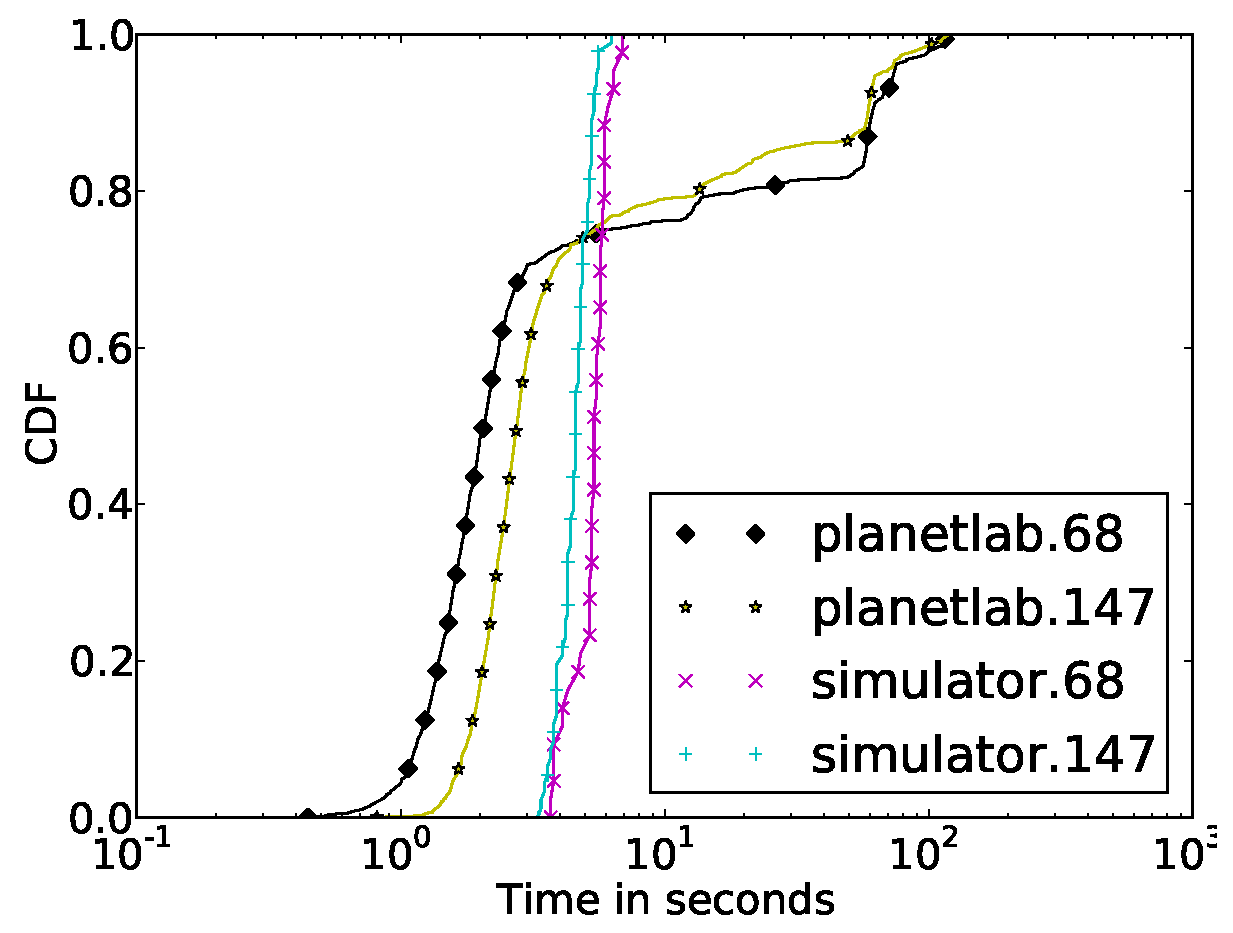
\includegraphics[width=4in]{figs/private.eps}
\caption[CDF of private overlay bootstrap time]{CDF (culmulative distribution
function) of the time to bootstrap a private overlay node in a private overlay
of the size stated in the legend using a public overlay consisting of 600
nodes.  Using a 100 ms delay like the simulator results in 9.2 and 9.3 seconds
for the analytical model for private network sizes of 68 and 147,
respectively.}
\label{fig:private_bootstrapping}
\end{figure}

Based upon the results presented in Figure~\ref{fig:private_bootstrapping}, the
bootstrapping time for the implementation performs better than the analytical
model, due to the simplicity of the analytical model and the small network
sizes.  It is of interest that while the simulator results tend to be in a well
defined range, the PlanetLab results have a few outliers with long bootstrap
times.  Some of the expected causes for this are churn in the system and state
machine timeouts in Brunet, though I have not considered this in much depth.

\subsection{Overhead of Pathing}

Much like the previous experiment, this verifies that the pathing technique has
negligible overheads for VPN usage.  To determine the overheads, two GroupVPNs
are deployed on resources on the same gigabit LAN (local area network).  To
measure latency and throughput, netperf experiments are run for 30 seconds, 5
times each on an unutilized network switch.  Other specifications of the
machine are ignored as the system without pathing is used as the baseline.  The
results, Table~\ref{tab:pathing}, indicate that the use of pathing presents
negligible overhead for both throughput and latency, justifying the use of this
approach to transparently deal with NAT and firewall traversal.

\begin{table}[ht]
\caption[Pathing overheads]{Pathing overheads}
\centering
\begin{tabular*}{\textwidth}{@{\extracolsep{\fill}}
l
S[table-format=1.3,table-number-alignment=right]
S[table-format=3.2,table-number-alignment=right]
@{}
}
\hline & 
\multicolumn{1}{c}{Latency (ms)} &
\multicolumn{1}{c}{Throughput (Mbit/s)} \\ \hline \hline
Standard & .303 & 225.27 \\ \hline
Pathing & .308 & 224.36 \\ \hline
\end{tabular*}
\label{tab:pathing}
\end{table}

\section{Security for the Overlay and the VPN}
\label{vpn:security}

Structured overlays are difficult to secure and a private overlay is not secure
if it provides no means to limit access to the system.  Malicious users can
pollute the DHT, send bogus messages, and even prevent the overlay from
functioning, rendering the VPN useless.  To address this in means that make
sense for VPNs and common users, I have employed a public key infrastructure
(PKI) to encrypt and authenticate both communication between peers as well as
communication across the overlay, called point-to-point (PtP) and end-to-end
(EtE) communication, respectively.

Use of a PKI (public key infrastructure) motivates from the ability to
authenticate without a third party, ideal for P2P use, unlike a key
distribution centers (KDC) used by other VPNs.  A PKI can use either
pre-exchange public keys or a certificate authority (CA) to sign public keys,
i.e., certificates.  Thus peers can exchange keys and certificates without
requiring a third-party to be online.

The reasons for securing PtP and EtE are different.  Securing PtP communication
prevents unauthorized access to the overlay, as peers must authenticate with
each other for every link created.  Though once authenticated, a peer can
perform malicious acts and since the overlay allows for routing over it, the
peer can disguise the origination of the malicious acts.  By also employing EtE
security, the authenticity of messages transferred through an overlay can be
verified.  Though EtE security by itself, will not prevent unauthorized access
into the overlay.  By employing both PtP and EtE, overlays can be secured from
uninvited guests from the outside and can identify malicious users on the
inside.  Implementing both leads to important questions: what mechanisms can be
used to implement both and what are the effects of both on an overlay and to a
VPN on an overlay.

\subsection{Implementing Overlay Security}

There are various types of PtP links, such as TCP and UDP sockets and relays
across individual nodes and the overlay.  EtE communication is
datagram-oriented in IPOP.  Traditional approaches of securing communication
such as IPsec are not convenient due to complexity, i.e., operating system
specific, portability constraints, and lack of common APIs.  Security protocols
that rely on reliable connections, such as SSL (secure sockets layer) or TLS
(transport layer security) are undesirable as well as they would require a
userspace implementation of reliable streams (akin to TCP).  As such, I have
implemented an abstraction called a security filter as presented in
Figure~\ref{fig:security_filter}, which enables nearly transparent use of
security libraries and protocols.  To this date, I have implemented both a
DTLS~\cite{dtls} (dtagram transport layer security) filter using the OpenSSL
implementation of DTLS as well as a protocol that reuses cryptographic
libraries provided by .NET that behaves similarly to IPsec.

A security filter has two components: the manager, and individual sessions or
filters.  While the individual sessions could act as filters by themselves, by
combining with a manager, they can be configured for a common purpose and
security credentials.  This approach enables the use of security to be
transparent to the other components of the system as the manager handles
session establishment, garbage collection of expired sessions, and revocation
of peers.

\begin{figure}
\centering
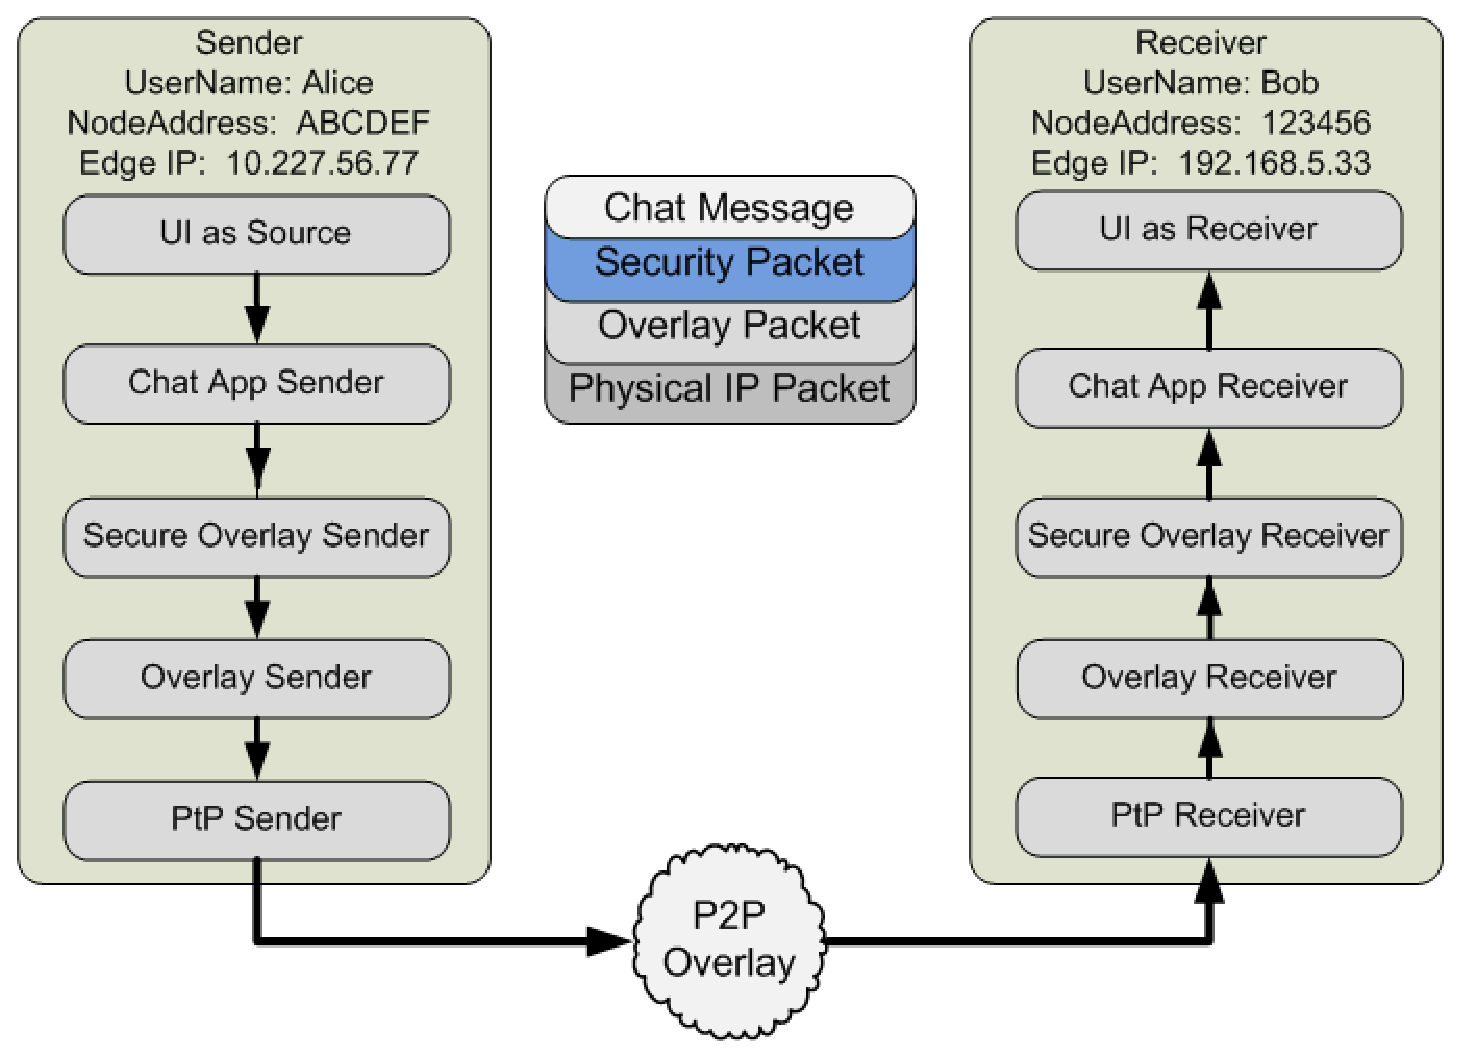
\includegraphics[width=6in]{figs/secure_sender_stack_generic.png.eps}
\caption[Security filter]{An example of the security filter abstraction used by
senders and receivers through an EtE secured chat application.  Each receiver
and sender use the same abstracted model and thus the chat application requires
only high-level changes, such as verifying the certificate used is Alice's and
Bob's, to support security.}
\label{fig:security_filter}
\end{figure}

Certificate embed identity of the owner, thus a signed certificate states that
the signer trusts that the identity is accurate.  In network systems, the
certificate uses the domain name to uniquely identify and limit the use of a
certificate.  When a CA signs the certificate, by including the domain name, it
ensures that users can trust that a certificate is valid, while used to secure
traffic to that domain.  Communication with another domain using the same
certificate will raise a flag and will result in the user not trusting the
certificate.  In environments with NATs, dynamic IP addresses, or portable
devices, typical of P2P systems, assigning a certificate to a domain name will
be a hassle as it constrains mobility and the type of users in the system.
Furthermore, most users are unaware of their IP address and changes to it.
Instead, a certificate is signed against the user's P2P address and unique user
name as delegated by the CA.  The purpose of the former is for efficiency of
revocation as discussed in Section~\ref{vpn:revocation}.  During the formation
of PtP links or while parsing EtE messages, the two nodes discover each other's
P2P addresses.  If the addresses do not match the address on the verified
certificate, the communication need not proceed further.  

Prior to trusting the security filter, the core software or the security filter
must ensure that the P2P address of the remote entity matches that of the
certificate.  In my approach, I did this by means of a callback, which presents
the underlying sending mechanism, EtE or PtP, and the overlay address stored in
the certificate.  The receiver of the callback can attempt to cast it into
known objects. If successful, it will compare the overlay address with the
sender type.  If unsuccessful, it ignores the request.  If any callbacks return
that the sender does not match the identifier, the session is immediately
closed.  Thus the security filter need not understand the sending mechanism and
the sending mechanism need not understand the security filter.

The last consideration comes in the case of EtE communication that provides an
abstraction layer.  For example, in the case of VPNs, where a P2P packet
contains an IP packet and thus a P2P address maps to a VPN IP address, a
malicious peer may establish a trusted link, but then hijack another user's IP
session.  As such, the application must verify that the IP address in the IP
packet matches the P2P address of the sender of the P2P packet.  In general, an
application address should be matched against a P2P address.

\subsection{Overheads of Overlay Security}

When applying an additional layer to a P2P system, there are overheads in terms
of time to connect with the overlay.  Other less obvious effects are
throughput, latency, and processing overheads, assuming that the P2P system
will be used over a wide area network, where the latency and throughput
limitations between two points will make the overhead of security negligible.
Though bootstrapping will be affected due to additional round trip messages
used for forming secure connections.

\begin{figure}[ht]
\centering
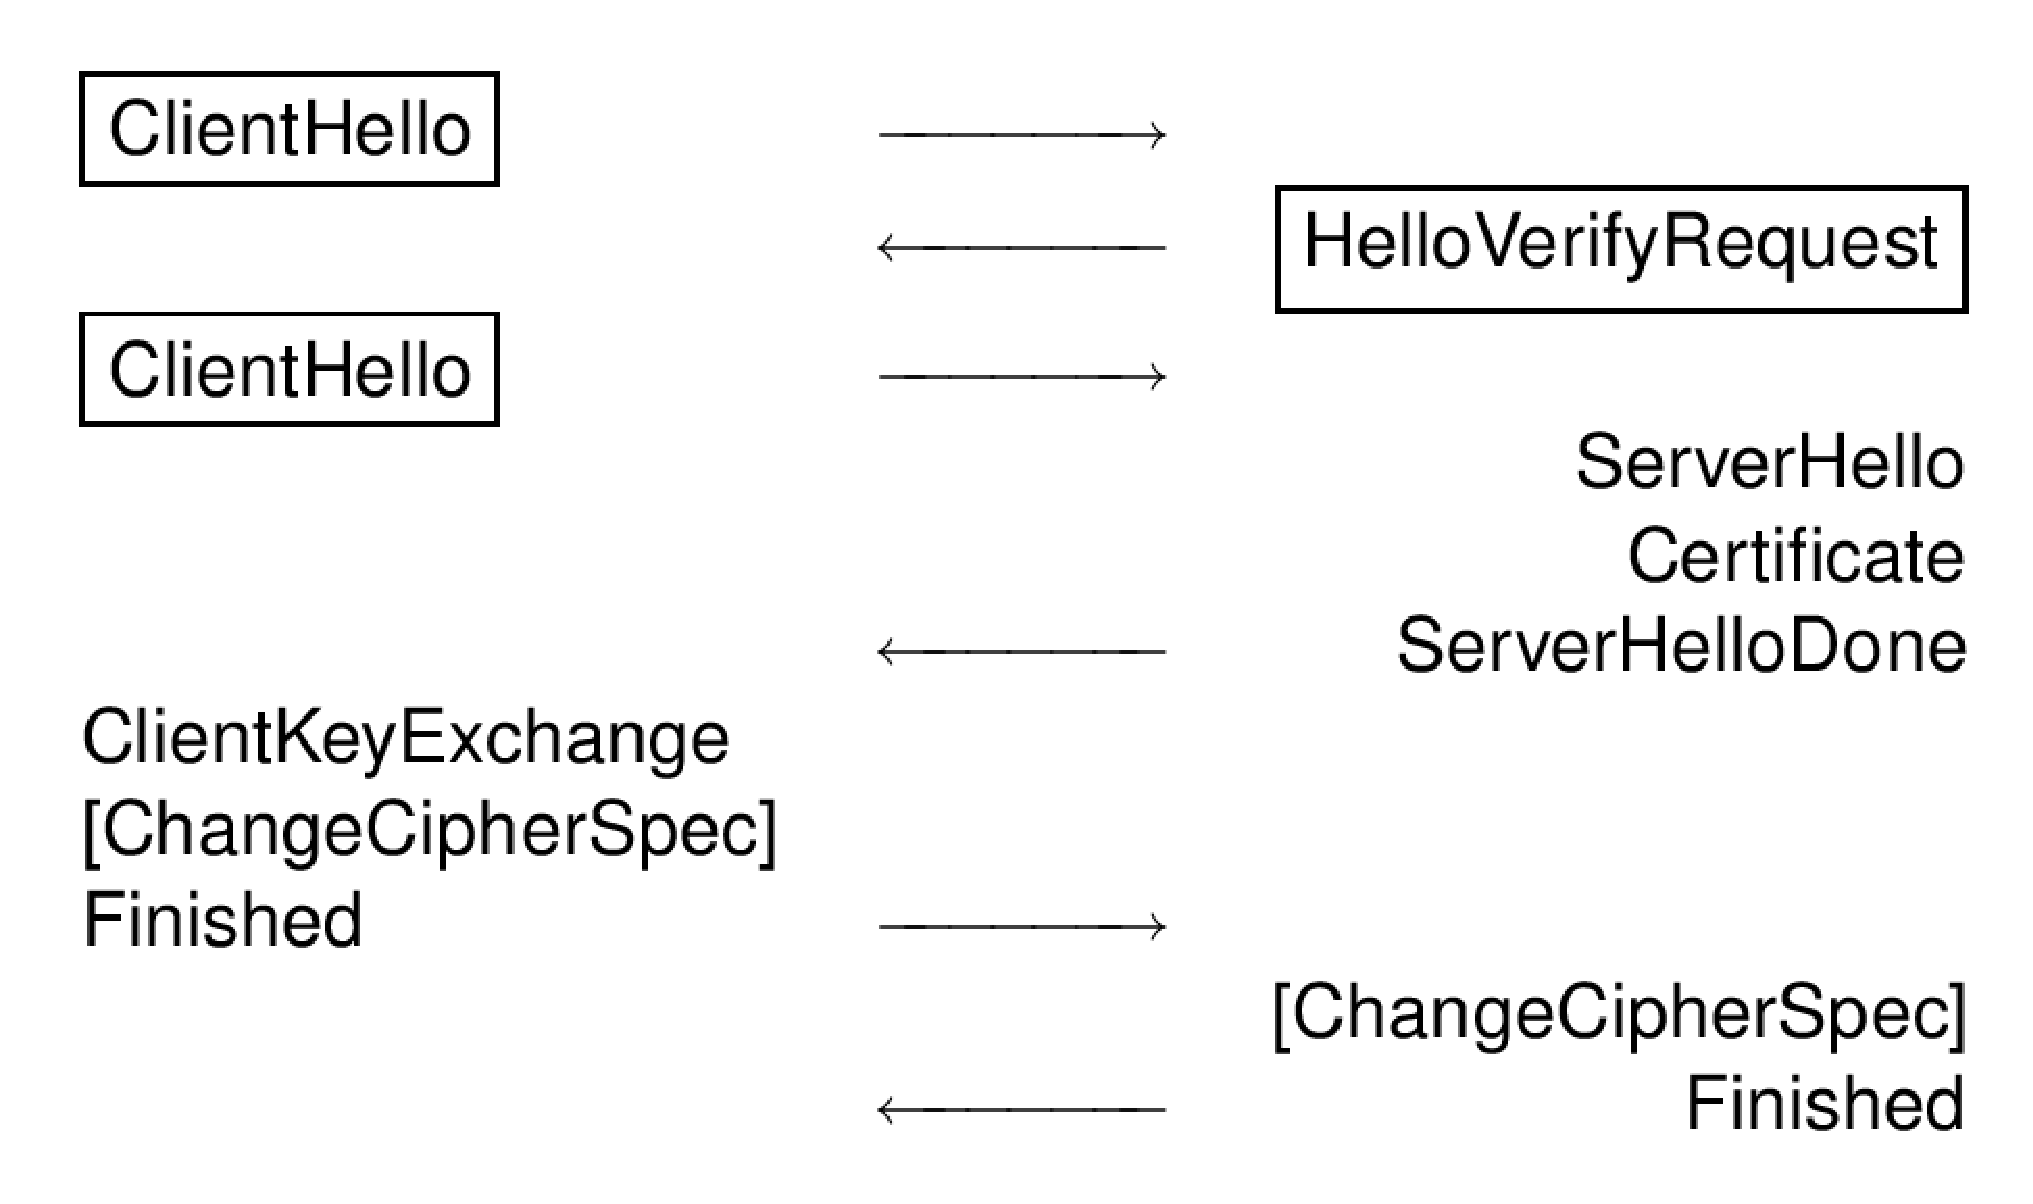
\includegraphics[width=4in]{figs/dtls.eps}
\caption[DTLS handshake]{DTLS handshake}
\label{fig:dtls}
\end{figure}

The DTLS handshake as presented in Figure~\ref{fig:dtls}, which consists of 6
messages or 3 round trips.  PtP security may very well have an effect on the
duration of overlay bootstrapping.  There even exists a possibility that with
more messages during bootstrap, the probability one drops is higher, which
could, in turn, also have an effect, though possibly negligible, on time to
connect.  To evaluate these concerns, I have employed both simulation and real
system experiments.

The following experiments use both simulation and PlanetLab deployment to
evaluate time to connect a new node to an existing resource.  Then another
experiment is performed to evaluate how long it takes to bootstrap various
sized overlays if all nodes join at the same time.  This experiment is only
feasible via simulation as attempting to reproduce in a real system is
extremely difficult due to how quickly the operations complete.

\subsubsection{Adding a Single Node}

This experiment determines how long it takes a single node to join an existing
overlay with and without DTLS security.  The experiment is performed using both
simulation and PlanetLab.  After deploying a set of nodes without security and
with security on PlanetLab, the network is crawled to determine the size of the
network.  In both cases, the overlay maintained an average size of around 600
nodes.  At which point, I connected a node 1,000, each time using a new,
randomly generated P2P address, thus connecting to a different point in the
overlay.  The experiment concludes as soon as the node has connected to the
peers in the P2P overlay immediately before and after it in the P2P address
space.  In the simulation, a new overlay is created and afterward a new node
joins, this is repeated 100 times.  The cumulative distribution functions
obtained from the different experiments are presented in
Figure~\ref{fig:add_one}.

\begin{figure}[ht]
\centering
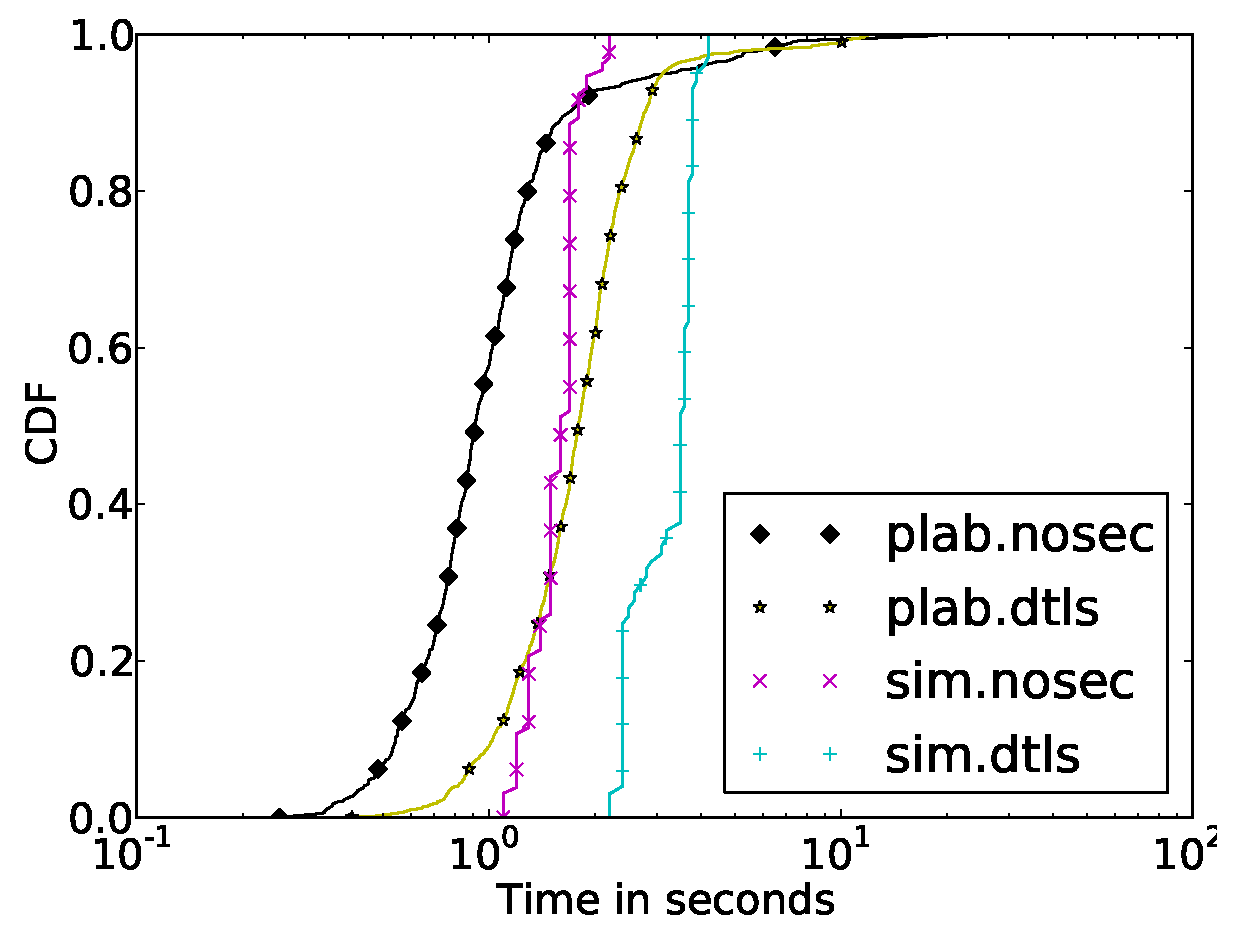
\includegraphics[width=4in]{figs/addone.eps}
\caption[Joining a secure overlay]{Time in seconds for a single node to join a
secure (dtls) and insecure (nosec) structured overlay, using both PlanetLab
(plab) and the Simulator (sim).} \label{fig:add_one}
\end{figure}

\subsubsection{Bootstrapping an Overlay}

The purpose of this experiment is to determine how quickly an overlay using
DTLS can bootstrap in comparison to one that does not given that there are no
existing participants.  Nodes in this evaluation are randomly given information
about 5 different nodes in the overlay and then all attempt to connect with
each other at the same time.  The evaluation completes after the entire overlay
has all nodes connected and in their proper position.  For each network size,
the test is performed 100 times and the average result is presented in
Figure~\ref{fig:bootstrap_eval}.

\begin{figure}[ht]
\centering
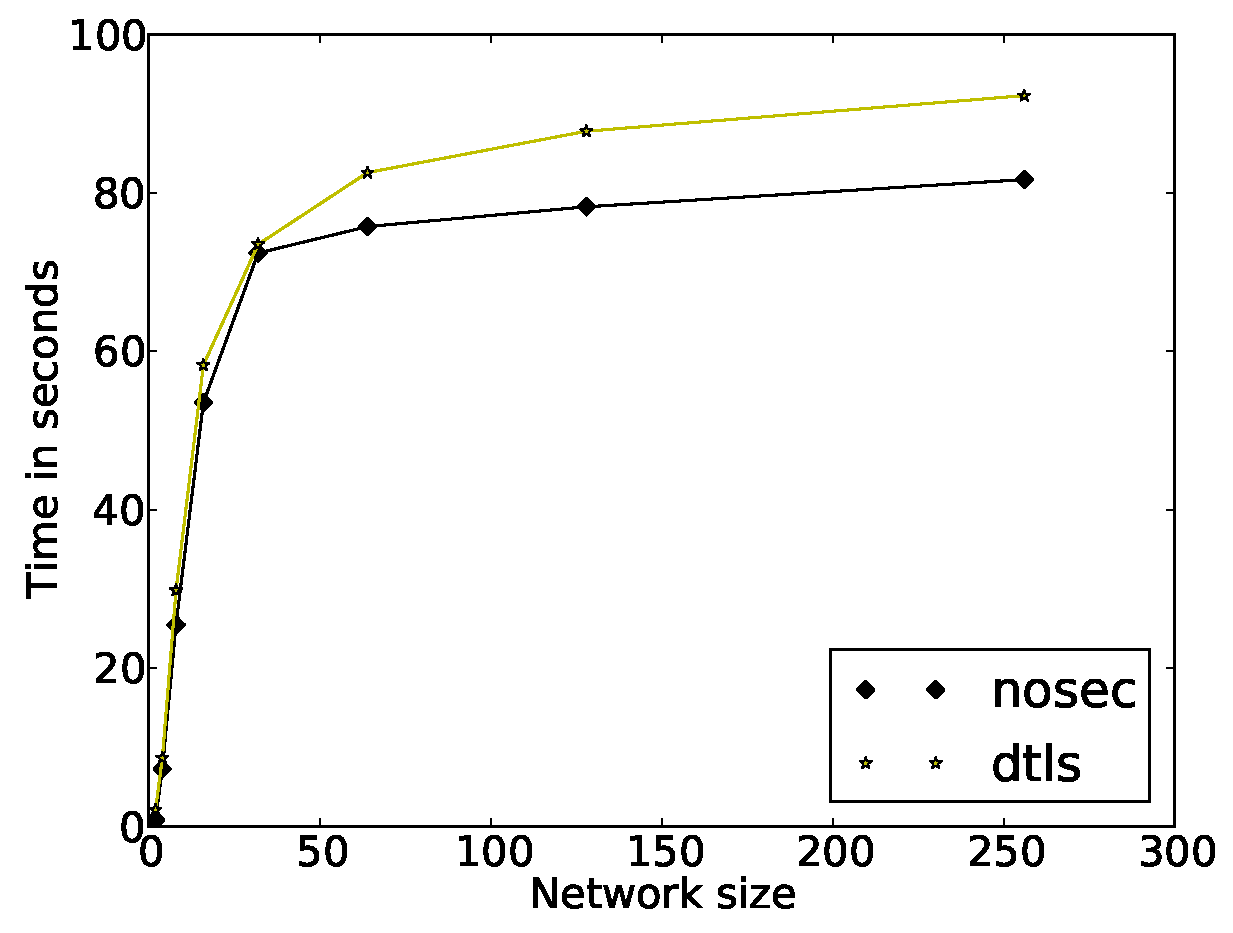
\includegraphics[width=4in]{figs/bootstrap_time.eps}
\caption[Bootstrapping a secure overlay]{Time in seconds for a secure (dtls)
and insecure (nosec) structured overlay to bootstrap, given that all nodes
bootstrap simultaneously.}
\label{fig:bootstrap_eval}
\end{figure}

\subsection{Discussion}

Both evaluations show that the overhead in using security is practically
negligible, when an overlay is small.  In the case of adding a single node, it
is clear that the simulation and deployment results agree, as the difference
between bootstrapping into an overlay with and without security remains nearly
the same.  Clearly this motivates the use of security if time to connect is the
most pressing question.

The time to bootstrap a secure overlay was not significantly more than that of
an insecure overlay.  What I realized is that complex connection handshaking,
as implemented in Brunet, seems to dominate connection establishment time.  For
example, in Brunet, two peers must communicate via the overlay prior to forming
a connection, and the system differentiates between bootstrapping connections
and overlay connections.  Thus even though a peer may have a bootstrapping
connection, it will need to go through the entire process to form an overlay
connection with a peer.  While this may lead to inefficiencies, this
simplification keeps the software more maintainable and easier to understand.

\section{Handling User Revocation}
\label{vpn:revocation}

Unlike decentralized systems that use shared secrets, in which the creator of
the overlay becomes powerless to control malicious users, PKIs enable their
creators to effectively remove malicious users.  Typical PKIs either use a
certificate revocation list (CRL) or online certificate verification protocols
such as Online Certificate Status Protocol (OCSP).  These approaches are
orthogonal to decentralized systems as they require a dedicated service
provider.  If the service provider is offline, an application can only rely on
historical information to make a decision on whether or not to trust a link.
In a decentralized system, these features can be enhanced so not to rely on a
single provider.  In this section, I present two mechanisms of doing so:
storing revocations in the DHT and performing overlay broadcast based
revocations.

\subsection{DHT Revocation}

A DHT can be used to provide revocation similar to that of OCSP or CRLs.
Revocations, a hash of the certificate and a time stamp signed by the CA, are
stored  are stored in the DHT at the key formed by the hashing of the
certificate.  In doing so, revocations will be uniformly distributed across the
overlay, not relying on any single entity.

The problem with the DHT approach is that it does not provide an event
notification for members currently communicating with the peer.  While peers
could continue to poll the DHT to determine a revocation, doing so is
inefficient.  Furthermore, a malicious peer, who has a valid but revoked
certificate could force every member in the overlay to query the DHT,
negatively affecting the DHT nodes storing the revocation.

\subsection{Broadcast Revocation}

Broadcast revocation uses a structured overlay based broadcast approach as
described in Appendix~\ref{broadcast}.  The form of broadcast can be used to
perform to notify the entire overlay immediately about a new revocation.  It is
important to note, that the message needs to be delivered locally prior to
forwarding, so that peers who have a connection to the malicious peer, will end
the connection prior to accidentally forwarding the message to the peer by
receiving and acting upon the revocation prior to forwarding the message.  

\subsection{Evaluation of Broadcast}

I performed an evaluation on the broadcast using the simulation to determine
how quickly peers in the overlay would receive the message.  The tested network
sizes ranged from 2 to 256 in powers of 2.  The tests were evaluations were
performed 100 times for each network size.  The CDF of hops for each node are
presented in Figure~\ref{fig:broadcast_cdf}.  The results make it quite clear that
the broadcast can efficiently distribute a revocation much more quickly than
$\log(N)$ time.

\begin{figure}[ht]
\centering
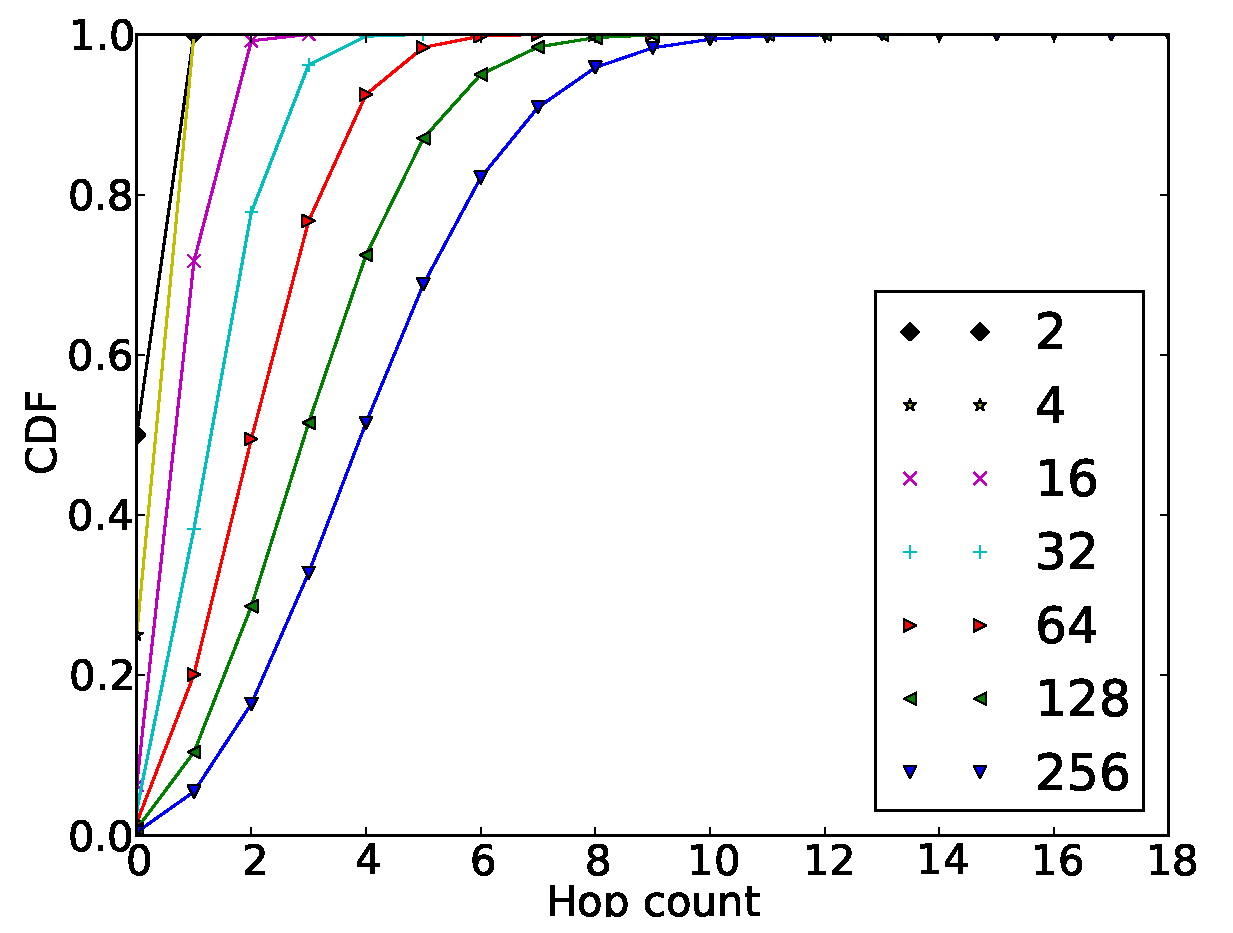
\includegraphics[width=4in]{figs/broadcast.eps}
\caption[Overlay broadcast time]{Overlay broadcast time CDF.}
\label{fig:broadcast_cdf}
\end{figure}

\subsection{Discussion}

In contrast to the DHT solution, broadcast revocation occurs only once and
leaves no state behind.  Thus the broadcast is not a complete solution, as new
peers connected to the overlay or those who missed the broadcast message will
be unaware of a revocation.  Furthermore, if an overlay is shared by many VPNs,
it may prevent overlay broadcasting or itself may be inefficient.

The DHT solution by itself may also not sufficient as revocations may be lost
over time as the entries must have their leases renewed in the DHT.  To address
this condition, each peer maintains a local CRL and the owner of the overlay
can occasionally send updates to the CRL through an out of band medium, such as
e-mail.  A better long term solution may be the use of a gossip protocols so
that peers can share their lists with each other during bootstrapping phases.

A key assumption in using these is that a Sybil~\cite{Sybil}, or collusion
attack, is difficult in the secured overlay.	 If a Sybil attack is successful,
both a DHT and broadcast revocation may be unsuccessful, though peers could fix
this problem by obtaining the CRL out of band.  In addition, previous
work~\cite{secure_routing} has described decentralized techniques to limit the
probability of such attacks from occurring.  In my approach, the use of central
authority to review certificate requests can be used to limit a single user
from obtaining too many certificates as well as ensuring uniform distribution
of that user's P2P addresses, further hampering the likelihood of a Sybil
attack.  The ability to automate this is left as future work.

One way to mitigate Sybil attacks using the broadcast approach is to bundle
colluding offenders into a single revocation message.  That would prevent those
from colluding together to prevent each other's revocations.  Furthermore,
while not emphasized above, revocation in my system revokes by user name and
not individual certificates.  Combined these two components limit Sybil attacks
against broadcast.

\section{Managing and Configuring the VPN}
\label{vpn:groupvpn}

While the PKI model applies to P2P overlays, actual deployment and maintenance
of security credentials can be too complex to manage, particularly for
non-experts.  Most PKI-enabled systems require the use of command-line
utilities and lack methods for assisting in the deployment of certificates and
policing users.  My solution to facilitate use of PKIs for non-experts is a
partially-automated PKI reliant on a group-based Web interface distributable in
forms of Joomla add-ons as well as a virtual machine appliance.  In this
environment, groups can share a common Web site, while each group has their own
unique CA.  Although this does not preclude other methods of CA interaction,
experience has shown that it provides a model that is satisfactory for many use
cases.

Group-based Web 2.0 sites enable low overhead configuration of collaborative
environments.  The roles in a group environment can be divided into
administrators and users.  Users have the ability to join and create groups;
whereas administrators define network parameters, can accept or deny join
requests, remove users, and promote other users to administrators.  By applying
this to a VPN, the group environment provides a simple to use wrapper around
PKI, where the administrators of the group act as the CA and the members have
the ability to obtain signed certificates.  

Elaborating further, when a user joins a group, the administrator can enable
automatic signing of certificates or require prior review; and when peers have
overstayed their welcome, an administrator can revoke their certificate by
removing them from the group.  Revocations are handled as described in
Section~\ref{vpn:revocation}.  In the context of GroupVPN systems, a user
revocation list as opposed to a CRL simplifies revocation, since users and not
individual certificates will be revoked.

Registered users who create groups become administrators of their own groups.
When a user has been accepted into a group by its administrator, they are able
to download VPN configuration data from the Web site.  Configuration data is
loaded by the GroupVPN during its configuration process to specify IP address
range, namespace, and security options.  The configuration data also stores a
shared secret, which uniquely identifies the user, enabling the Web site to
automatically sign the certificate (or enqueue it form manual signing,
depending on the group's policy).  Certificate requests consist of sending a
public key and a shared secret over an HTTPS connection to the web server.
Upon receiving the signed certificate, peers are able to join the private
overlay and GroupVPN, enabling secure communication amongst the VPN peers.  The
entire bootstrapping process, including address resolution and communication
with a peer, is illustrated in Figure~\ref{fig:groupvpn}.

\begin{figure}[ht]
\centering
\includegraphics[width=3.5in,angle=-90]{figs/groupvpn.ps}
\caption[Bootstrapping a new GroupVPN]{Bootstrapping a new GroupVPN}
\label{fig:groupvpn}
\end{figure}

There are many ways of implementing and hosting the Web site.  For example,
Google offers free hosting of Python web applications through Google Apps, an
option available if the user owns a domain.  Alternatively, the user could host
the group site on a public virtual network. In this case, peers interacting
with the GroupVPN would need to connect with the public virtual network in
order to create an account, get the configuration data, and retrieve a signed
certificate, at which point they could disconnect from it.  This does not
preclude the use of other social mediums nor a central site dedicated to the
formation of many GroupVPNs.  Many GroupVPNs can share a single site, so long
as the group members trust the site to host the CA private key.

\section{Leveraging Trust from Online Social Networks}

Groups are very useful for coordinating a set of individuals when a subset of
them can be used to establish trust amongst them all.  However, groups can lack
clear and concise individuality and limit independence from the collective.  As
noted in~\cite{socialvpn}, trust can be leveraged from existing social networks
to create trust in other domains.  Much like that of a social network, a VPN
consists of trusted links, tying the two together produced the
SocialVPN~\cite{socialvpn}.  In this work, I along with my fellow researchers
implemented a prototype for SocialVPN, which exemplifies the utility of my
approaches in handling security both in terms of trust and session
establishment as well as endpoint configuration of the VPN.

Besides the content described in the following subsections, namely establishing
identity and trust as well as address allocation and discovery, SocialVPN
reuses existing components already provided in IPOP, such as secure link
establishment, endpoint configuration, and packet handling.  Even the
functionality used by SocialVPN for address allocation and discovery builds
upon existing abstractions already provided by IPOP.

\subsection{Architecture}

SocialVPN leverages the online social network to establish trust and exchange
certificates.  Thus a social network must provide a means for an external
application to determine friendships and store arbitrary data into the social
network.  The arbitrary data in this case would be the certificate that can be
used to find a peer in the network overlay and verify its identity.  The
certificate consists of the peer's social network information and P2P address.
Thus once a peer has connected to a social network the first time, it need only
be repeated to obtain the latest information.  Existing certificates remain
valid until the friendship has ended for the certificate cache has been
explicitly flushed.

Once a peer has a certificate, connections are immediately established with all
``friends'' that are currently connected to the overlay.  As new peers come
online, they establish connections with those already there.  Due to potential
network problems, this may not occur, and so all members of SocialVPN will
occasionally check the liveness of peers not connected to the overlay.  Because
online peers have an active connection, there is no need to explicitly monitor
their state.  When they go offline, the connection will be broken and can be
represented to the user appropriately.

The motivation in establishing connections immediately comes from two purposes:
no overhead in bootstrapping on demand connections and better ability to
distribute IP multicast and broadcast packets.  Using the traditional IPOP
style to establish a direct connection can take somewhere between several
hundreds of milliseconds up to several seconds, which may be disappointing to
users who have used centralized VPNs that have much faster connection
establishment.  Because there currently exists no support for efficient
broadcast / multicast message distribution inside SocialVPN, maintaining an
active link to all peers allows a peer to push that message to all their peers
without having to establish a new trusted link first.

\subsection{Leveraging Trust From Facebook}

Trust or friendships already established in Facebook used a now deprecated
technology that allowed desktop applications access to Facebook.  Certificate
exchange relied upon a web-based data store component provided by Facebook,
which was presented as a database.  When SocialVPN first contacts Facebook, it
would add the current certificate, if it did not exist and then download
certificates for all friends that it did not already have.  Because a user
might have more than one instance of SocialVPN running, the database was
designed to allow the user to store multiple certificates and to clear their
certificates.  As mentioned earlier, each certificate contains the friends P2P
address, which allows a peer to discover a remote peer and establish a trusted,
direct VPN link with them.

Unfortunately, Facebook's interface was poorly constructed and no longer
exists.  Each application had to embed in itself private key information to
authenticate itself with Facebook.  A malicious attacker could easily discover
this and change the stored data to suit their needs.  While Facebook never gave
a reason for shutting down the desktop application component of their system,
this is a probable reason.

As an alternative, I developed a web application, which was used for a short
period of time to replace the desktop application; however, this was fraught
with problems.  Unlike the desktop application that only required trust with
Facebook, the web application required hosting a third-party web site to
support the system.  The trust model is not significantly different as the
administrator for the application has access to the trusted material
regardless, it simply meant another centralized component.  These complications
led to the development of an XMPP-based SocialVPN.

\subsection{Leveraging Trust from XMPP}

Unlike Facebook, XMPP is a well standardized, open system with many individual
members contributing compatible services.  Thus if one of them decides to break
from the XMPP specification, users can easily migrate to another service
provider.  After the unfortunate incident with Facebook, this open aspect was
much more attractive to SocialVPN as a research project

As discussed in Section~\ref{bs:xmpp_bootstrapping}, XMPP is primarily used as
an open protocol instant messenger service.  Though it has support for
exchanging binary messages through ``IQ.'' When a peer using SocialVPN connects
to XMPP, they are informed of their friends that are online.  Each friend has a
unique name in the form ``username@domain/resource.'' When a peer receives this
message, they can determine if that friend is using SocialVPN by the resource
name.  If the peer is discovered to be using SocialVPN they will exchange
certificates and proceed to establish trusted links in the overlay. 

\subsection{Address Allocations and Discovery}

In creating a VPN where links are defined by social networking relationships,
the mechanisms for IP address allocation via the DHT do not apply well.  A
social networking based VPN will form an overlay that does not need to rely on
a structured overlay and so to do without requires a new addressing scheme.
Additionally, attempting to place all peers inside a social network within an
IP address range, especially IPv4, is fraught with problems~\cite{rfc5684}.
Namely that it can be difficult to find a common address space for all peers
inside a VPN, which can be made even more difficult if those peers use another
VPN product.

The concept employed in SocialVPN is to place each user inside their own
private address space independent of other users.  Each friend of that peer has
a unique IP address unbeknownst to them inside this address space.  The IP is
mapped to the users P2P address.  Then through the use of packet translation,
IP addresses are transparently changed as the packet is transferred between
peers.  Prior to delivery, the packet's destination address is converted to the
peers own pre-defined IP address and the source address is based upon a mapping
stored inside a hashtable that maps P2P address to IP address.  Only trusted
peers will have a mapping like this.

\section{Related Work}
\label{vpn:related_work}

\subsection{VPNs}

Hamachi~\cite{hamachi} is a centralized P2P VPN provider using the web site for
authentication, peer discovery, and connection establishment.  While the
Hamachi protocol claims to support various types of
security~\cite{hamachi_security}, the implementation appears to only support
the KDC requiring that all peers establish trusted relationship through the
central website.  The Hamachi approach makes it easy for users to deploy their
own services, but places limitations on network size, uses a proprietary
security stack, and does not allow independent VPN deployments.  In contrast,
my approach presents a completely decoupled environment allowing peers to start
using the shared system to bootstrap private overlays and migrate away without
cost if need be.  Furthermore my approach relies only on a central server to
obtain the certificate otherwise, it is decentralized.  In Hamachi, if the
central server goes offline, no new peers can join the VPN.

Campagnol VPN~\cite{campagnol} provides similar features to Hamachi: a P2P VPN
that relies on a central server for rendezvous or discovery of peers.  The key
differences between Hamachi and Campagnol is that Campagnol is free and does
not provide a service; users msut deploy their own rendezvous service.  The
authors of Campagnol also state that the current approach limits the total
number of peers sharing a VPN to 100 so not to overload the rendezvous service.
The current implementation does not support a set of rendezvous nodes, though
doing so would make the approach much more like ours.  In addition, the system
relies on traditional distribution of a CRL to handle revocation.

Tinc~\cite{tinc} is a decentralized VPN requiring users to manually organize an
overlay with support for finding optimal paths.  In comparison to my approach,
Tinc does not automatically handle churn in the VPN.  If a node connecting two
separate pieces of the VPN overlay goes offline, the VPN will be partitioned
until a user manually creates a link connecting the pieces.  Furthermore, Tinc
does not form direct connections for improved latency and throughput reasons,
thus members acting as routes in the overlay incur the price of acting as
packet forwarders.

The last VPN, I discuss is the most similar to IPOP, its called N2N~\cite{n2n}.
N2N uses unstructured p2p techniques to form an Ethernet based VPN.  While
their approach, like ours, has built-in NAT traversal, it requires that users
deploy their own bootstrap and limits security to a single pre-shared key for
the entire VPN, thus users cannot be revoked.  Since N2N provides Ethernet,
users must provide their own mechanism for IP address allocation, while
discovery utilizes overlay broadcasting.  Thus there are concerns that as
systems get larger, N2N may not be very efficient.

\subsection{P2P Systems}

BitTorrent~\cite{bittorrent_security}, a P2P data sharing service,  supports
stream encryption between peers sharing files.  The purpose of BitTorrent
security is to obfuscate packets to prevent traffic shaping due to packet
sniffing. Thus BitTorrent security uses a weak stream cipher, RC4, and lacks
peer authentication as symmetric keys are exchanged through an unauthenticated
Diffie-Hellman process.

Skype~\cite{skype} provides decentralized audio and video communication to over
a million concurrent users.  While Skype does not provide documentation
detailing the security of its system, researchers~\cite{skype_auth,
skype_overview} have discovered that Skype supports both EtE and PtP security.
Though similar to Hamachi, Skype uses a KDC and does not let users setup their
own systems.

As of December 2009, the FreePastry group released an SSL enabled
FreePastry~\cite{pastry}.  Though relatively little is published regarding
their security implementation, the use of SSL prevents its application for use
in the overlay and for overlay links that do not use TCP, such as relays and
UDP.  Thus their approach is limited to securing environments that are not
behind NATs and firewalls that would prevent direct TCP links from forming
between peers.
